\section{RQ2 (Provenance): How the Score Was Produced}
\label{sec:rq2}

A benchmark score is the output of a pipeline, and the released pipeline leaves choices open at four stages: which representation of the telemetry the method reads, what happens when the method fails, how invalid outputs enter the denominator, and how cases are weighted and scored.
RQ1 read each subsystem difference as a property of the method and the subsystem; this section asks which choices of the released pipeline produced it.
The duplicated header of \cref{sec:design-protocol} is one such choice's effect, a subsystem anomaly that disappears once the input is fixed.
For each stage we compare the reference configuration of \cref{sec:design-protocol} with one alternative on the same cases and the same methods, and record for every pair and subsystem whether $\Delta_s$ changes sign and whether the comparison's reversal status changes (\cref{tab:factors}).
The stages are not equal: the first two produced opposite conclusions with CIs excluding zero on both sides; the last two moved, on \openrca, only differences that were already close to zero.

\begin{table}[t]
\caption{Pipeline stages that change comparison conclusions. Comp.: comparisons (one method pair on one subsystem); Sign: comparisons whose $\Delta_s$ changes sign; Rev.: comparisons that are a reversal under exactly one of the two conditions. All pairs include probes and shipped baselines; --: no published pair has outputs under both conditions. Seed: the three-seed mean of a randomized method against any single seed, over the comparisons that involve such a method (\cref{sec:rq2-denominator}).}
\label{tab:factors}
\footnotesize
\setlength{\tabcolsep}{4pt}
\begin{tabular*}{\textwidth}{@{\extracolsep{\fill}}llrrrrrr@{}}
\toprule
 & & \multicolumn{3}{c}{Published methods} & \multicolumn{3}{c}{All pairs} \\
\cmidrule(lr){3-5} \cmidrule(lr){6-8}
Factor & Family & Comp. & Sign & Rev. & Comp. & Sign & Rev. \\
\midrule
Input representation & RCAEval RE1 & 12 & 5 & 1 & 42 & 16 & 8 \\
 & RCAEval RE2 & -- & -- & -- & 18 & 5 & 7 \\
\addlinespace
Silent failure (duplicated header) & RCAEval RE1 & 30 & 2 & 2 & 84 & 3 & 4 \\
\addlinespace
Denominator (valid outputs only) & RCAEval RE1 & 30 & 0 & 0 & 84 & 0 & 0 \\
 & RCAEval RE2 & 71 & 1 & 1 & 146 & 2 & 2 \\
 & OpenRCA & 12 & 0 & 0 & 60 & 0 & 0 \\
 & PetShop & 40 & 0 & 0 & 220 & 0 & 0 \\
\addlinespace
Fault re-weighting & RCAEval RE1 & 30 & 0 & 0 & 84 & 0 & 0 \\
 & RCAEval RE2 & 71 & 0 & 0 & 146 & 0 & 0 \\
 & OpenRCA & 12 & 3 & 3 & 60 & 13 & 15 \\
 & PetShop & 40 & 1 & 1 & 220 & 2 & 1 \\
\addlinespace
Scoring (strict $=1$) & OpenRCA & 12 & 4 & 0 & 60 & 11 & 8 \\
\addlinespace
Scoring ($\geq 0.5$) & OpenRCA & 12 & 0 & 0 & 60 & 3 & 3 \\
\bottomrule
\end{tabular*}

\end{table}

\subsection{Input Representation}
\label{sec:rq2-input}

RE1-SS and RE1-TT can be read from the raw export or from the reduced table (\cref{sec:design-protocol}), and the two readings do not rank the methods the same way.
\Cref{fig:input} shows each method's accuracy under both.
\baro falls from \InSSBaroSimple to \InSSBaroRaw on SS and from \InTTBaroSimple to \InTTBaroRaw on TT, and \circa from \InSSCircaSimple to \InSSCircaRaw and from \InTTCircaSimple to \InTTCircaRaw, while \alertcount and \cdmin improve on TT and \ediag and \rcd barely move.
The raw export is not a uniform penalty; it reorders the methods.
The release does not state which table its reported numbers use, and a reader who runs it as shipped obtains the raw numbers.

\begin{figure}[t]
\centering
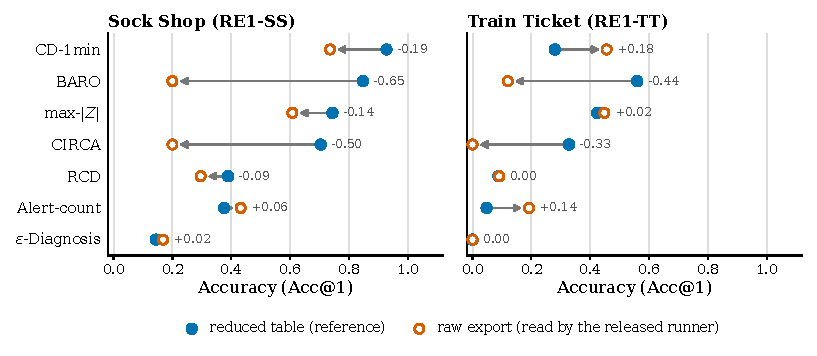
\includegraphics[width=\textwidth]{figures/fig3_input_dumbbell.pdf}
\caption{RE1 accuracy of each method on the reduced table (the reference) and on the raw export that the released runner reads.}
\label{fig:input}
\end{figure}

Among published methods, \InReOnePubSign of the \InReOnePubComp SS and TT comparisons change sign, the largest share at any stage.
\circa leads \rcd by \InCircaRcdSSOk \InCircaRcdSSOkCI on SS and \InCircaRcdTTOk \InCircaRcdTTOkCI on TT with the reduced tables; with the raw exports \rcd leads, by \InCircaRcdSSRaw \InCircaRcdSSRawCI and \InCircaRcdTTRaw \InCircaRcdTTRawCI.
All four intervals exclude zero: two analyses of the same released cases, each a literal reading of the release, report opposite conclusions with the same apparent support.
On SS the best published method changes from \baro to \rcd.
The raw exports add \InReOnePubRevRaw reversals among published pairs (\InReOnePubRevCIRaw with CI support) that are absent with the reduced tables; \InReOnePubRevRawOB of them is on OB, whose data are the same under both conditions, because the pooled sign of \circa vs \rcd changes (\cref{tab:factors} counts the SS and TT comparisons).
Among all pairs \InReOneAllSign of \InReOneAllComp comparisons change sign, each condition showing reversals the other lacks: the input representation replaces one set of conclusions with another.
RE2 ships the same two kinds of table, and there the runner reads the reduced one; the raw table changes \InReTwoSign of \InReTwoComp comparisons among the methods we could run on it.

\subsection{Silent Failures}
\label{sec:rq2-defect}

A method that fails inside the pipeline but returns a complete ranking leaves no trace on the leaderboard; the ranking is scored like any other.
Both failures found in \cref{sec:design-protocol} are of this kind.
Under the drifted dependency, \causalrca returns the input column order on every case we tested, so a comparison that involves it on the release as shipped compares the column order of the input file, not the method.
The duplicated header in 50 RE1-OB tables has an effect we can measure, because \circa and \ediag run on the same cases before and after the fix.
On the files as shipped, \circa's accuracy on RE1-OB is \DefCircaShipped; after dropping the duplicated column it is \DefCircaFixed (\DefCircaShippedAff and \DefCircaFixedAff on the 50 affected cases).
As shipped, \causalrca beats \circa on OB by \DefCrCircaShipped \DefCrCircaShippedCI, a CI-supported reversal of \circa's pooled lead; after the fix the difference is \DefCrCircaFixed \DefCrCircaFixedCI, and \circa vs \rcd on OB changes from \DefCircaRcdShipped to \DefCircaRcdFixed.
Of \DefPubComp comparisons between published methods on RE1, \DefPubSign change sign, and the shipped files produce \DefPubRevShipOnly reversals (\DefPubRevCIShipOnly with CI support) that disappear after the fix.
Neither failure raises an error or lowers coverage; the one check that reveals both is whether a method's ranking equals the order of the input columns.

\subsection{Denominator and Reported Numbers}
\label{sec:rq2-denominator}

\NCovBelowOne of \NCovCells method-by-subsystem cells (seeds counted separately) have coverage below 1, for method-specific reasons: \tracerca and \microrank fail on the same 17 RE2-TT cases with a missing-key error, leaving \CovTraceValid valid outputs of 90; \ediag returns three metrics per query, none of which belongs to the candidate set in most \openrca Telecom queries (\CovEdTelValid of \CovEdTelN valid); and one seed of \causalrca learns an empty graph in 43 RE2-TT cases (\CovCrSeedOneValid valid).
Scoring valid outputs only, instead of all cases, changes \DenReTwoPubSign of \DenReTwoPubComp comparisons between published methods on RE2 and \DenReTwoAllSign of \DenReTwoAllComp among all pairs, all on RE2-TT (\circa vs \tracerca moves from \DenCircaTraceAll to \DenCircaTraceValid), and none of the \DenOtherComp comparisons in the other families.
Two things a reported number does not state matter when it is compared with a published one: the denominator and the seed.
Our \tracerca and \microrank outputs match every per-fault value that \rcaeval reports for RE2-TT (18 cells each, within 0.01) only if the 17 failed cases are dropped, although the paper's definition of the metric divides by all cases.
Over all cases, \tracerca's \acc is \CovTraceAll instead of the reported 0.66.
% src: .research/verifications/2026-09-27-re2-rcaeval-table6.md
\causalrca's code defines a seed but never applies it, and on RE2-TT, where \rcaeval reports 0.22, our three seeds give \CovCrReTwoTTSeedZero, \CovCrReTwoTTSeedOne, and \CovCrReTwoTTSeedTwo.
Taking any single seed instead of the three-seed mean changes the sign of \SeedReOnePubSign of the \SeedReOnePubComp comparisons between published methods that involve a randomized method on RE1, \SeedReTwoPubSign of \SeedReTwoPubComp on RE2, and \SeedOpenrcaPubSign of \SeedOpenrcaPubComp on \openrca (last row of \cref{tab:factors}).

\subsection{Fault Composition}
\label{sec:rq2-fault}

A pooled score also mixes fault types, which are not equally frequent in every subsystem.
We re-weight each subsystem so that the fault classes it shares with the rest of its family count equally.
Both \rcaeval releases contain the same number of cases for every fault type in every application, so no comparison there changes.
\openrca's four subsystems share only CPU and network faults; restricting each subsystem to these and weighting them equally changes the sign of \FwOpenrcaPubSign of \FwOpenrcaPubComp comparisons between published methods and \FwOpenrcaAllSign of \FwOpenrcaAllComp overall, none with a CI that excludes zero; on \petshop (latency and availability faults), \FwPetshopPubSign of \FwPetshopPubComp and \FwPetshopAllSign of \FwPetshopAllComp change.

\subsection{Scoring Rule}
\label{sec:rq2-scoring}

\openrca's official score gives partial credit.
Counting only fully correct answers changes the sign of \ScStrictPubSign of \ScStrictPubComp comparisons between published methods (\ScStrictAllSign of \ScStrictAllComp overall); requiring a score of at least 0.5 changes \ScHalfPubSign and \ScHalfAllSign.
All \ScStrictPubToZero sign changes between published methods under the strict rule are differences that become exactly zero, and none changes a reversal status (\cref{tab:factors}): on Market-1, \baro, \rcd, and \ediag score \ScMktOneBaroStrict, \ScMktOneRcdStrict, and \ScMktOneEdiagStrict under the strict rule and \ScMktOneBaroPartial, \ScMktOneRcdPartial, and \ScMktOneEdiagPartial with partial credit.
Under the strict rule the published methods are indistinguishable on that subsystem; the ordering reported under partial credit comes entirely from partially correct answers.
Among all pairs, \ScStrictAllRevNonzero of the reversal-status changes remain non-zero differences and \ScStrictAllRevToZero is a reversal that becomes a tie.
Every method's score on \openrca lies between \ScOpenrcaOfficialMin and \ScOpenrcaOfficialMax under the official rule and between \ScOpenrcaStrictMin and \ScOpenrcaStrictMax under the strict one, so the differences a scoring rule can move there are of this size.
Where scores are not at the floor the rule moves more: on RE2-OB, \baro's accuracy is \BaroAccReTwoOB at top-1 and \BaroReTwoOBAccThree at top-3 (\cref{sec:rq1-release}).

\subsection{Reading the Four Stages Together}
\label{sec:rq2-summary}

The first two stages changed conclusions between published methods with CI support; the last two changed, on \openrca, the sign only of differences that were close to zero in the reference analysis, or turned them into ties.
Both silent failures were found in \rcaeval, the one family whose released runner we could execute as shipped; \openrca releases no runner for these methods, and we found none in \petshop's harness.
The largest provenance effect we measured is a choice of the release rather than of the runner: which metric kinds it records (\cref{sec:rq1-release}) changed \baro's accuracy by as much as the input representation did.
The denominator, the fault weighting, and the scoring rule are choices every benchmark makes, and they are the ones a reader can usually see.
An audit should therefore start with what is least visible, which table the runner reads, which metric kinds it contains, and whether rankings equal the input column order, then ask how invalid outputs enter the denominator, and only then turn to the weighting and the scoring rule.
